\chapter{Empreendedorismo Social e Negócios de Impacto Territorial}
\label{cap:unid1_cap05}

\noindent\tagAV{AV1 (30\%)}\ \tagCritico

\vspace{6pt}

\begin{capObjetivos}
Ao concluir este capítulo, você deverá ser capaz de:
\begin{itemize}[leftmargin=1.4em, itemsep=3pt]
  \item Aplicar o \textbf{Quadro PCDO} (Austin, Stevenson \& Wei-Skillern, 2006) para contrastar o empreendedorismo comercial e o empreendedorismo social em suas dimensões estruturais.
  \item Avaliar empreendimentos segundo os critérios nacionais dos \textbf{Negócios de Impacto} (Aliança pelos Investimentos e Negócios de Impacto).
  \item Construir e quantificar uma \textbf{Teoria da Mudança} (Insumos $\to$ Atividades $\to$ \textit{Outputs} $\to$ \textit{Outcomes} $\to$ Impacto), calculando o \textbf{SROI} com ajuste de peso morto e deslocamento.
  \item Analisar o \textbf{Espectro do Capital} e instrumentos financeiros híbridos, como \textbf{Títulos de Impacto Social (SIBs)} e \textbf{\textit{Blended Finance}}.
  \item Diagnosticar o risco de \textbf{\textit{mission drift}} (desvio de missão) e problematizar a \textbf{financeirização do social} e os limites do hibridismo organizacional.
\end{itemize}
\end{capObjetivos}

\begin{capRevisao}
No Capítulo~4, discutimos como o Estado Empreendedor, os NITs e as políticas orientadas por missões criam condições macroinstitucionais para a inovação. Contudo, muitas falhas sociais e ambientais nos territórios não são resolvidas apenas por agências estatais ou por empresas orientadas exclusivamente ao lucro acionário. Neste Capítulo~5, investigamos as organizações híbridas que buscam equacionar sustentabilidade financeira e transformação socioambiental mensurável.
\end{capRevisao}

\etapa{3}{Fundamentação Teórica, Teoria da Mudança e Modelagem}

\begin{boxSimbolo}[Vocabulário Conceitual e Símbolos do Capítulo]
\renewcommand{\arraystretch}{1.18}
\begin{tabular}{@{}p{2.4cm} p{12.0cm}@{}}
  PCDO & Quadro analítico: \textit{People} (Pessoas), \textit{Context} (Contexto), \textit{Deal} (Negócio) e \textit{Opportunity} (Oportunidade), articulados pela Proposição de Valor Social (SVP). \\
  \textit{Outputs} & Produtos ou entregas diretas e imediatas das atividades (ex.: cisternas instaladas). \\
  \textit{Outcomes} & Mudanças ou benefícios reais percebidos pelo público-alvo (ex.: redução de doenças hídricas). \\
  $SROI$ & Retorno Social sobre o Investimento (\textit{Social Return on Investment}). \\
  $DW,\ DL$ & Fatores de ajuste de impacto: \textit{Deadweight} (peso morto) e \textit{Displacement} (deslocamento). \\
  $k_{blend}$ & Custo médio ponderado de capital em operações de \textit{Blended Finance}. \\
  SIBs & \textit{Social Impact Bonds} (Títulos / Contratos de Impacto Social com pagamento por resultado). \\
  \textit{Mission Drift} & Desvio gradual da missão social em favor de metas financeiras ou públicos de maior renda. \\
\end{tabular}
\end{boxSimbolo}

\subsection{O Quadro PCDO: Empreendedorismo Comercial vs. Social}

Em trabalho seminal, James Austin, Howard Stevenson e Jane Wei-Skillern (2006) adaptaram o modelo de empreendedorismo de Sahlman para explicar o que distingue o empreendedorismo social do comercial. O \textbf{Quadro PCDO} organiza essa análise ao articular quatro variáveis interdependentes, correspondentes a \textbf{Pessoas} (\textit{People}), \textbf{Contexto} (\textit{Context}), \textbf{Negócio ou Acordo} (\textit{Deal}) e \textbf{Oportunidade} (\textit{Opportunity}), tendo no centro a \textbf{Proposição de Valor Social (SVP)}. Enquanto no empreendimento comercial os contratos entre sócios, investidores e clientes tendem a ser padronizados pelo retorno financeiro, no empreendimento social a SVP precisa alinhar beneficiários que muitas vezes não têm capacidade de pagamento integral com terceiros financiadores, como o Estado, doadores ou clientes de subsídio cruzado.

\renewcommand{\arraystretch}{1.20}
\small
\begin{tabularx}{\textwidth}{@{}p{2.4cm} X X@{}}
  \toprule
  \rowcolor{etIndigo}
  \textcolor{white}{\bfseries Dimensão} & \textcolor{white}{\bfseries Empreendedorismo Comercial} & \textcolor{white}{\bfseries Empreendedorismo Social} \\
  \midrule
  \textbf{Oportunidade (O)} & Mercado em crescimento capaz de gerar retorno econômico apropriável. & Falha de mercado ou vulnerabilidade socioambiental persistente (demanda social). \\
  \rowcolor{bgGray}
  \textbf{Pessoas (P)} & Remuneração competitiva de mercado e participação acionária (\textit{equity}) para atrair talentos. & Mobilização de recursos humanos frequentemente dependente de propósito, voluntariado e redes comunitárias. \\
  \textbf{Contexto (C)} & Regulação setorial, juros e concorrência de mercado. & Marco regulatório público, políticas sociais, cultura territorial e vulnerabilidade institucional. \\
  \rowcolor{bgGray}
  \textbf{Negócio / Deal (D)} & Acordos contratuais padronizados entre investidores, sócios e clientes pagantes. & Relações complexas com múltiplos \textit{stakeholders} (beneficiários frequentemente distintos dos pagadores). \\
  \bottomrule
\end{tabularx}
\normalsize

\subsection{Critérios dos Negócios de Impacto}

No Brasil, a \textbf{Aliança pelos Investimentos e Negócios de Impacto} estabelece quatro pilares articulados para diferenciar um Negócio de Impacto genuíno de ações filantrópicas ou de práticas isoladas de responsabilidade social corporativa. O primeiro pilar é a \textbf{intencionalidade}, segundo a qual o propósito explícito de resolver um problema socioambiental consta na estratégia central da organização. O segundo exige uma \textbf{atividade-fim geradora de impacto}, garantindo que o benefício coletivo decorra diretamente do produto ou serviço principal comercializado, sem se restringir a doações acessórias de parte do lucro.

Além desses dois critérios de propósito, o empreendimento precisa estruturar um \textbf{modelo de negócio financeiramente sustentável}, capaz de gerar receitas próprias (via venda a usuários, empresas ou poder público) que cubram os custos operacionais e permitam ganhar escala sem dependência perpétua de doações. Complementando essa arquitetura, o quarto pilar combina \textbf{impacto mensurável e governança}, exigindo métricas claras de acompanhamento de resultados e mecanismos estatutários que protejam a missão social ao longo do tempo diante de pressões comerciais.

\subsection{Teoria da Mudança e Espectro do Capital}

A \textbf{Teoria da Mudança (ToC)} explicita a cadeia causal pela qual os recursos mobilizados geram transformação territorial, conforme representado no encadeamento a seguir.
\[
\textbf{Insumos} \longrightarrow \textbf{Atividades} \longrightarrow \textbf{\textit{Outputs} (Entregas)} \longrightarrow \textbf{\textit{Outcomes} (Resultados)} \longrightarrow \textbf{Impacto Sistêmico}
\]
Enquanto os \textit{outputs} medem o volume operacional produzido pela organização, como o número de oficinas ministradas ou de kits solares entregues, os \textit{outcomes} mensuram a mudança efetiva na vida do público atendido, expressa no aumento da renda líquida familiar, na redução de internações ou na autonomia energética.

No financiamento dessas iniciativas, o \textbf{Espectro do Capital} posiciona as fontes de recursos em um contínuo que vai desde a \textbf{filantropia tradicional}, voltada exclusivamente ao retorno social com aceitação de perda total do principal, passando por investimentos \textbf{\textit{impact-first}} (que priorizam o impacto e aceitam retorno financeiro abaixo do mercado) e \textbf{\textit{finance-first}} (que exigem retorno de mercado com tese de impacto), até o \textbf{investimento tradicional} focado exclusivamente no retorno ajustado ao risco. A Figura~\ref{fig:teoria_mudanca_espectro} ilustra essa articulação entre a cadeia causal da Teoria da Mudança e o posicionamento dos instrumentos financeiros ao longo do Espectro do Capital.

\begin{figure}[H]
  \centering
  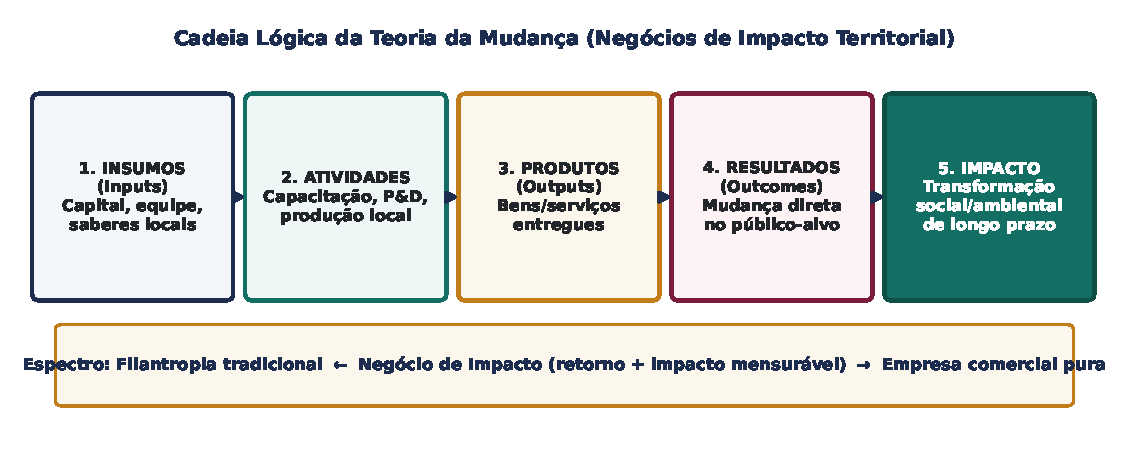
\includegraphics[width=0.94\textwidth]{figures/fig05_teoria_mudanca_espectro.pdf}
  \caption{Integração entre a cadeia causal da Teoria da Mudança e o posicionamento dos instrumentos financeiros ao longo do Espectro do Capital.}
  \label{fig:teoria_mudanca_espectro}
\end{figure}

\subsection{Instrumentos Financeiros Híbridos e Contraponto Crítico}

Dois instrumentos financeiros híbridos ganham destaque na agenda contemporânea de impacto por conectarem diferentes faixas do Espectro do Capital. O primeiro é o \textbf{\textit{Blended Finance} (Finanças Mistas)}, que combina estrategicamente capital concessional ou filantrópico (capaz de absorver primeiras perdas ou aceitar juros zero) com capital comercial privado, reduzindo o risco percebido e destravando investimentos em setores ou territórios periféricos. O segundo instrumento corresponde aos \textbf{Títulos de Impacto Social (SIBs / Contratos de Impacto Social)}, arranjo contratual em que investidores privados financiam antecipadamente uma intervenção social executada por um operador especializado, cabendo ao poder público reembolsar o investidor com remuneração pactuada apenas se metas independentes de \textit{outcome} forem comprovadamente atingidas.

\begin{boxConceito}[Contraponto Crítico: \textit{Mission Drift}, Financeirização do Social e Limites do Hibridismo]
A literatura crítica aponta três tensões estruturais que acompanham os negócios de impacto. A primeira é o \textbf{\textit{Mission Drift} (Desvio de Missão)}, que ocorre quando, diante da pressão de investidores por liquidez e margem, a empresa híbrida migra gradualmente para clientes de maior poder aquisitivo e abandona o público vulnerável de menor capacidade de pagamento. A segunda tensão envolve a \textbf{financeirização do social}, uma vez que os SIBs podem transformar direitos sociais constitucionais (educação, saúde, saneamento) em ativos financeiros sujeitos à lógica de retorno de curto prazo e à seleção adversa (\textit{cream-skimming}, priorizando casos mais fáceis de atingir a meta). A terceira tensão envolve os \textbf{limites do hibridismo}, pois nem todo problema territorial comporta um modelo de receita pagante; em situações de extrema pobreza ou provisão de bens públicos puros, a ação estatal direta e a economia solidária permanecem insubstituíveis.
\end{boxConceito}

\begin{boxFormula}[Modelagem Quantitativa: SROI Ajustado e Custo Ponderado em \textit{Blended Finance}]
\textbf{1. Valor de Impacto Líquido e Retorno Social sobre o Investimento ($SROI$):}
Para evitar superestimar o impacto atribuindo ao projeto mudanças que ocorreriam de qualquer maneira (\textit{deadweight}, $DW$) ou que apenas transferiram o problema para outro local (\textit{displacement}, $DL$), calcula-se o benefício líquido ajustado:
\[
V_{liq} = V_{bruto} \times (1 - DW) \times (1 - DL)
\]
A razão $SROI$ e o $SROI$ líquido percentual são dados por:
\[
SROI_{razao} = \frac{V_{liq}}{I_{total}} \qquad \text{e} \qquad SROI_{liq} = \frac{V_{liq} - I_{total}}{I_{total}}
\]

\textbf{2. Custo Médio Ponderado de Capital em \textit{Blended Finance} ($k_{blend}$):}
Sendo $w_i$ a fração de capital da camada $i$ (com $\sum w_i = 1$) e $k_i$ seu respectivo custo anual:
\[
k_{blend} = \sum_{i=1}^{n} w_i \cdot k_i
\]
\end{boxFormula}

\etapa{4}{Exemplos Resolvidos e Estudos de Caso Comentados}

\begin{boxExemplo}{5.1}{Aplicação do Quadro PCDO: \textit{Fintech} Urbana vs. Banco Comunitário Digital}
\passoEnunciado{Compare uma \textit{fintech} comercial de crédito pessoal em capital metropolitano com uma \textit{fintech} de impacto territorial voltada a microempreendedoras informais no Recôncavo Baiano.}
\passoDados{A \textit{fintech} comercial opera com garantia em folha ou histórico de crédito formal, captando em fundos de \textit{venture capital}. O negócio de impacto utiliza dados alternativos de comércio local, agentes comunitários de crédito e capital inicial subsidiado.}
\passoPedido{Estruturar a comparação pelas quatro dimensões do Quadro PCDO (Austin et al., 2006) e identificar a principal vulnerabilidade do negócio de impacto.}
\passoMetodo{Mapeamento comparativo qualitativo nas dimensões Oportunidade, Pessoas, Contexto e \textit{Deal}.}
\passoContas{
\begin{itemize}[leftmargin=1.4em, itemsep=2pt]
  \item \textbf{Oportunidade:} comercial busca margem sobre tomadores bancarizados; impacto busca inclusão produtiva de desbancarizados com redução de juros extorsivos.
  \item \textbf{Pessoas:} comercial remunera com \textit{stock options} de mercado; impacto combina equipe técnica com agentes locais remunerados por vínculo territorial.
  \item \textbf{Contexto:} impacto depende de regulação do Banco Central para sociedades de crédito direto e da informalidade da renda rural/urbana local.
  \item \textbf{Negócio (\textit{Deal}):} comercial tem relação bilateral investidor--cliente; impacto precisa conciliar retorno ao fundo concessional com taxas acessíveis às microempreendedoras.
\end{itemize}
}
\passoResposta{A principal vulnerabilidade do negócio de impacto no Quadro PCDO reside no \textit{Deal}: se o custo de captação subir, há pressão para elevar os juros às tomadoras, desencadeando \textit{mission drift}.}
\passoVerificacao{O Quadro PCDO explicita por que métricas comerciais padrão não capturam a complexidade de contratos com múltiplos interesses territoriais.}
\end{boxExemplo}

\begin{boxExemplo}{5.2}{Teoria da Mudança e Cálculo de SROI Ajustado em Saneamento Rural}
\passoEnunciado{Um negócio de impacto instalou sistemas modulares de tratamento de água cinza (biofiltros) em 200 residências rurais de um território semiárido, permitindo reuso agrícola em quintais produtivos.}
\passoDados{Investimento total do ciclo: $I_{total} = \reais{500.000,00}$. A valoração monetária bruta dos benefícios em 3 anos (economia de água comprada em carro-pipa, produção de hortaliças e redução de gastos com doenças de veiculação hídrica) somou $V_{bruto} = \reais{1.600.000,00}$. Auditoria independente estimou peso morto (\textit{deadweight}) de $DW = 20\%$ e efeito de deslocamento (\textit{displacement}) de $DL = 10\%$.}
\passoPedido{Distinguir um \textit{output} de um \textit{outcome} do projeto e calcular o benefício líquido ajustado ($V_{liq}$), o $SROI_{razao}$ e o $SROI_{liq}$.}
\passoMetodo{Aplicação da cadeia de Teoria da Mudança e das fórmulas de $SROI$ com descontos multiplicativos de $DW$ e $DL$.}
\passoContas{
1. Distinção causal: \textit{output} = 200 biofiltros instalados; \textit{outcome} = redução da incidência de diarreia infantil e aumento da segurança alimentar via reuso.\\
2. Benefício líquido ajustado:
\[
V_{liq} = 1.600.000 \times (1 - 0{,}20) \times (1 - 0{,}10) = 1.600.000 \times 0{,}80 \times 0{,}90 = 1.600.000 \times 0{,}72 = \reais{1.152.000,00}
\]
3. Indicadores de $SROI$:
\[
SROI_{razao} = \frac{1.152.000}{500.000} = 2{,}304 \approx 2{,}30 \qquad \text{e} \qquad SROI_{liq} = \frac{1.152.000 - 500.000}{500.000} = \frac{652.000}{500.000} = 1{,}304\ (130{,}4\%)
\]
}
\passoResposta{Cada $\reais{1,00}$ investido gerou $\reais{2,30}$ de valor socioambiental líquido ($SROI$ líquido de $130{,}4\%$).}
\passoVerificacao{O desconto de $28\%$ acumulado ($1 - 0{,}72$) evita a inflação artificial de resultados típica de relatórios promocionais sem grupo de controle.}
\end{boxExemplo}

\begin{boxExemplo}{5.3}{Estruturação de \textit{Blended Finance} para Bioeconomia Regional}
\passoEnunciado{Uma cooperativa de beneficiamento de frutas nativas necessita de $\reais{4.000.000,00}$ para ampliar sua câmara fria e linha de polpas. O crédito bancário comercial exige taxa de $14\%$ ao ano, inviabilizando o fluxo de caixa do projeto, que suporta no máximo $8\%$ ao ano.}
\passoDados{Estruturou-se uma operação de \textit{Blended Finance} com três camadas: (1) $30\%$ de doação/subvenção filantrópica a custo $k_1 = 0\%$ a.a.; (2) $40\%$ de fundo de investimento de impacto (\textit{impact-first}) a $k_2 = 6\%$ a.a.; (3) $30\%$ de empréstimo bancário comercial a $k_3 = 14\%$ a.a.}
\passoPedido{Calcular o custo médio ponderado de capital ($k_{blend}$) da operação e verificar se o projeto torna-se financeiramente viável.}
\passoMetodo{Cálculo da média ponderada $k_{blend} = w_1 k_1 + w_2 k_2 + w_3 k_3$.}
\passoContas{
\[
k_{blend} = (0{,}30 \times 0\%) + (0{,}40 \times 6\%) + (0{,}30 \times 14\%) = 0\% + 2{,}4\% + 4{,}2\% = 6{,}6\%\ \text{a.a.}
\]
Em termos monetários anuais sobre $\reais{4.000.000,00}$, o custo financeiro cai de $\reais{560.000,00}$ (a $14\%$) para $\reais{264.000,00}$ (a $6{,}6\%$).
}
\passoResposta{O custo ponderado reduz-se para $k_{blend} = 6{,}6\%$ a.a., abaixo do teto de $8\%$ suportado pela cooperativa, viabilizando o investimento.}
\passoVerificacao{O capital filantrópico atuou como alavanca catalítica para atrair o capital comercial sem sufocar a capacidade de pagamento do empreendimento territorial.}
\end{boxExemplo}

\begin{boxExemplo}{5.4}{Modelagem de Título de Impacto Social (SIB) em Educação Técnica}
\passoEnunciado{Um governo estadual analisa a contratação de um Título de Impacto Social (SIB) para reduzir a evasão escolar no ensino médio técnico de uma região industrial periférica.}
\passoDados{Custo público estimado por aluno evadido (perda fiscal e programas assistenciais futuros): $\reais{8.000,00}$. Meta contratual de retenção comprovada por auditoria: $250$ estudantes adicionais mantidos até a formatura. Capital privado antecipado pelos investidores ao operador social: $\reais{1.200.000,00}$. Cláusula de remuneração caso a meta seja integralmente cumprida: pagamento total de $120\%$ do capital investido (principal + $20\%$ de retorno).}
\passoPedido{Calcular a economia bruta gerada ao Estado se a meta for atingida, o pagamento máximo ao investidor e a economia líquida para os cofres públicos.}
\passoMetodo{Comparação entre o benefício fiscal evitado ($N \times \text{Custo unitário}$) e o desembolso contratual por resultado.}
\passoContas{
1. Economia pública bruta com a retenção dos $250$ estudantes:
\[
E_{bruta} = 250 \times 8.000 = \reais{2.000.000,00}
\]
2. Pagamento máximo ao investidor privado em caso de sucesso integral:
\[
P_{invest} = 1.200.000 \times 1{,}20 = \reais{1.440.000,00}
\]
3. Economia líquida efetiva para o Estado:
\[
E_{liq} = 2.000.000 - 1.440.000 = \reais{560.000,00}
\]
}
\passoResposta{Se a meta for cumprida, o investidor recebe $\reais{1.440.000,00}$ e o Estado obtém economia líquida de $\reais{560.000,00}$; se a meta falhar, o Estado não desembolsa o pagamento por resultado.}
\passoVerificacao{Apesar da atratividade fiscal, o gestor deve auditar o risco de \textit{cream-skimming}, garantindo que o operador não selecione apenas estudantes com menor risco prévio de evasão.}
\end{boxExemplo}

\begin{boxExemplo}{5.5}{Diagnóstico Quantitativo de \textit{Mission Drift}}
\passoEnunciado{Uma clínica popular de telemedicina, criada como negócio de impacto para atender comunidades rurais sem cobertura especializada, passou por uma rodada de capital de risco (\textit{finance-first}) no Ano 1.}
\passoDados{
\textbf{Ano 1:} $8.000$ atendimentos a pacientes de baixa renda (ticket $\reais{50,00}$) e $500$ atendimentos a planos empresariais de alta renda (ticket $\reais{200,00}$).\\
\textbf{Ano 3:} $6.000$ atendimentos a baixa renda (ticket $\reais{50,00}$) e $3.000$ atendimentos a planos empresariais (ticket $\reais{200,00}$).
}
\passoPedido{Calcular a receita total e a participação percentual do público-alvo vulnerável na receita e no volume de atendimentos entre o Ano 1 e o Ano 3, diagnosticando se houve \textit{mission drift}.}
\passoMetodo{Decomposição de receita por segmento ($R = Q \times P$) e cálculo de participação relativa.}
\passoContas{
\textbf{Ano 1:}\\
Receita baixa renda $= 8.000 \times 50 = \reais{400.000,00}$. Receita alta renda $= 500 \times 200 = \reais{100.000,00}$.\\
Receita total $= \reais{500.000,00}$. Participação da baixa renda na receita $= 400.000 / 500.000 = 80{,}0\%$.\\
\textbf{Ano 3:}\\
Receita baixa renda $= 6.000 \times 50 = \reais{300.000,00}$. Receita alta renda $= 3.000 \times 200 = \reais{600.000,00}$.\\
Receita total $= \reais{900.000,00}$. Participação da baixa renda na receita $= 300.000 / 900.000 \approx 33{,}3\%$.
}
\passoResposta{Embora o faturamento tenha crescido $80\%$ (de $\reais{500\text{ mil}}$ para $\reais{900\text{ mil}}$), o atendimento ao público vulnerável caiu de $8.000$ para $6.000$ consultas e sua participação na receita despencou de $80{,}0\%$ para $33{,}3\%$, confirmando \textit{mission drift}.}
\passoVerificacao{O subsídio cruzado só protege a missão quando a receita do segmento de alta renda expande o atendimento à base vulnerável, e não quando a substitui.}
\end{boxExemplo}

\etapa{5}{Armadilhas Conceituais e Erros Mais Comuns}

\begin{boxErro}[Erro 1: Confundir \textit{Output} com \textit{Outcome} na Teoria da Mudança]
Entregar $500$ cartilhas educativas ou realizar $40$ cursos é apenas um \textit{output} (volume de atividade). O \textit{outcome} exige comprovar o que mudou no território após a entrega (por exemplo, quantos agricultores adotaram a técnica e aumentaram sua produtividade líquida).
\end{boxErro}

\begin{boxErro}[Erro 2: Chamar Qualquer Projeto de Responsabilidade Social Corporativa (RSC) de Negócio de Impacto]
Uma mineradora ou banco que destina $1\%$ do lucro para patrocinar uma orquestra local pratica filantropia ou RSC, não um Negócio de Impacto. No Negócio de Impacto, a geração de valor socioambiental está no núcleo da atividade comercial principal.
\end{boxErro}

\begin{boxErro}[Erro 3: Ignorar Peso Morto (\textit{Deadweight}) no Cálculo de SROI]
Atribuir $100\%$ da melhoria observada ao empreendimento sem estimar o que teria acontecido na ausência da intervenção (tendência natural, políticas paralelas) superestima o SROI e compromete a credibilidade da avaliação perante investidores e o setor público.
\end{boxErro}

\begin{boxErro}[Erro 4: Tratar o SROI como Taxa Interna de Retorno Financeira (TIR)]
Um $SROI$ de $3{,}00$ não significa que o negócio possui caixa livre para pagar dividendos de $200\%$. O $SROI$ monetiza benefícios sociais e ambientais difusos (saúde, carbono evitado, coesão) que muitas vezes não entram no caixa da empresa.
\end{boxErro}

\etapa{6}{Exercícios Propostos (Básicos, Intermediários e Objetivos)}

\textbf{Parte A, Exercícios Básicos (Conceituação e Identificação)}

\textbf{1.} Explique a função central da Proposição de Valor Social (SVP) no Quadro PCDO de Austin, Stevenson e Wei-Skillern (2006).
\espacoResolucao[1.8cm]

\textbf{2.} Liste os quatro critérios essenciais definidos pela Aliança pelos Investimentos e Negócios de Impacto para caracterizar um Negócio de Impacto.
\espacoResolucao[1.8cm]

\textbf{3.} Em um projeto de capacitação digital para jovens de periferias urbanas, dê um exemplo de \textit{insumo}, um de \textit{output} e um de \textit{outcome}.
\espacoResolucao[1.8cm]

\textbf{4.} O que diferencia o investimento \textit{impact-first} do investimento \textit{finance-first} ao longo do Espectro do Capital?
\espacoResolucao[1.8cm]

\textbf{5.} Defina \textit{mission drift} (desvio de missão) e indique uma cláusula de governança capaz de preveni-lo.
\espacoResolucao[1.8cm]

\textbf{Parte B, Exercícios Intermediários (Modelagem e Análise Quantitativa)}

\textbf{6.} Um negócio de reciclagem inclusiva investiu $I_{total} = \reais{400.000,00}$ e gerou benefícios brutos estimados em $V_{bruto} = \reais{1.250.000,00}$ (economia de aterro sanitário e aumento de renda de catadores). Estudos apontam $DW = 12\%$ e $DL = 0\%$. Calcule $V_{liq}$, $SROI_{razao}$ e $SROI_{liq}$.
\espacoResolucao[2.0cm]

\textbf{7.} Calcule o custo médio ponderado de capital ($k_{blend}$) de um fundo territorial de $\reais{10\text{ milhões}}$ composto por: $20\%$ de recursos filantrópicos a $0\%$ a.a., $50\%$ de capital \textit{impact-first} a $5\%$ a.a. e $30\%$ de dívida bancária a $15\%$ a.a.
\espacoResolucao[2.0cm]

\textbf{8.} Um Título de Impacto Social (SIB) visa reduzir internações evitáveis por hipertensão em idosos. Cada internação evitada economiza $\reais{4.500,00}$ ao SUS. A meta é evitar $400$ internações com aporte privado de $\reais{1.000.000,00}$ e pagamento máximo de $\reais{1.300.000,00}$ em caso de sucesso. Calcule a economia líquida para o sistema público.
\espacoResolucao[2.0cm]

\textbf{9.} Analise criticamente o risco de \textit{cream-skimming} (seleção dos casos mais fáceis) em Contratos de Impacto Social na área de empregabilidade juvenil. Como a métrica contratual pode ser desenhada para neutralizar esse viés?
\espacoResolucao[2.0cm]

\textbf{10.} Uma escola técnica privada de impacto cobra mensalidade reduzida para estudantes de baixa renda e mensalidade integral para empresas conveniadas (subsídio cruzado). Em dois anos, a diretoria reduz as bolsas de baixa renda de $60\%$ para $25\%$ para acelerar o retorno aos sócios. Elabore um parecer avaliando se o modelo ainda atende aos critérios de Negócio de Impacto.
\espacoResolucao[2.0cm]

\textbf{Parte C, Questões Objetivas (Estilo Exame / Concurso, A a E)}

\textbf{11.} No Quadro PCDO (Austin et al., 2006), uma das distinções fundamentais entre o empreendedorismo social e o empreendedorismo comercial reside na dimensão \textit{Deal} (Negócio/Acordo), porque no empreendedorismo social:
\begin{alternativas}
  \item Não existem contratos formais nem prestação de contas financeiras.
  \item Os beneficiários diretos do serviço frequentemente não possuem capacidade de pagamento integral, exigindo articulação com terceiros pagadores (Estado, doadores ou subsídio cruzado).
  \item O lucro líquido é obrigatoriamente distribuído aos clientes finais na forma de dividendos.
  \item A oportunidade decorre exclusivamente de patentes de alta tecnologia protegidas no exterior.
  \item As pessoas envolvidas são proibidas por lei de receber remuneração salarial.
\end{alternativas}

\textbf{12.} Na estruturação de uma Teoria da Mudança, a sequência lógica correta do encadeamento causal é:
\begin{alternativas}
  \item \textit{Outcomes} $\to$ Insumos $\to$ \textit{Outputs} $\to$ Atividades $\to$ Impacto.
  \item Insumos $\to$ \textit{Outputs} $\to$ Atividades $\to$ Impacto $\to$ \textit{Outcomes}.
  \item Insumos $\to$ Atividades $\to$ \textit{Outputs} $\to$ \textit{Outcomes} $\to$ Impacto.
  \item Atividades $\to$ Insumos $\to$ Impacto $\to$ \textit{Outcomes} $\to$ \textit{Outputs}.
  \item Impacto $\to$ \textit{Outcomes} $\to$ \textit{Outputs} $\to$ Atividades $\to$ Insumos.
\end{alternativas}

\textbf{13.} Um fundo de \textit{Blended Finance} combina $40\%$ de capital concessional a $2\%$ a.a. com $60\%$ de capital comercial a $12\%$ a.a. O custo médio ponderado de capital ($k_{blend}$) dessa estrutura é:
\begin{alternativas}
  \item $6{,}0\%$ a.a.
  \item $7{,}0\%$ a.a.
  \item $8{,}0\%$ a.a.
  \item $9{,}2\%$ a.a.
  \item $10{,}0\%$ a.a.
\end{alternativas}

\textbf{14.} Sobre os Títulos de Impacto Social (SIBs) e a crítica à financeirização do social, assinale a alternativa \textbf{correta}:
\begin{alternativas}
  \item Nos SIBs, o poder público paga antecipadamente ao investidor privado, independentemente do alcance das metas sociais.
  \item O mecanismo de SIB elimina completamente os custos de auditoria e transação em políticas públicas.
  \item Uma crítica recorrente aos SIBs é o risco de \textit{cream-skimming}, isto é, a seleção de beneficiários mais fáceis de atender para garantir o retorno financeiro do contrato.
  \item Os SIBs são idênticos às debêntures incentivadas de infraestrutura rodoviária sem vínculo com indicadores de \textit{outcome}.
  \item O uso de SIBs impede a participação de organizações da sociedade civil como operadoras da intervenção.
\end{alternativas}

\textbf{15.} Em relação aos critérios da Aliança pelos Investimentos e Negócios de Impacto, uma empresa que vende refrigerantes ultraprocessados e destina $2\%$ de seu lucro para um projeto de hortas comunitárias classifica-se como:
\begin{alternativas}
  \item Negócio de Impacto pleno, pois possui intencionalidade filantrópica.
  \item Empresa tradicional com prática de investimento social privado / responsabilidade social corporativa, pois sua atividade-fim não gera o impacto socioambiental.
  \item Organização de economia solidária autogestionária.
  \item Título de Impacto Social com remuneração por \textit{outcome}.
  \item Fundo \textit{impact-first} de capital semente.
\end{alternativas}

\etapa{7}{Questões Autorais Estilo Pós-Graduação e Concursos}

\textbf{16. (Estilo Pós-Graduação em Gestão Social / Desenvolvimento Regional)} Discuta os limites do hibridismo organizacional diante da chamada ``tese da financeirização do social''. Em que situações territoriais o modelo de Negócio de Impacto (baseado em receita de mercado) é adequado e em quais situações a provisão pública estatal ou a economia solidária mostram-se superiores?
\espacoResolucao[2.2cm]

\textbf{17. (Estilo Concurso para Analista de Investimentos de Impacto, BNDES/BNB)} Uma aceleradora regional avalia dois projetos de impacto hídrico para receber capital em \textit{Blended Finance}. O Projeto X apresenta $SROI$ bruto de $4{,}0$, mas sem análise de peso morto e com receita dependente $90\%$ de doações. O Projeto Y apresenta $SROI$ líquido ajustado de $2{,}2$, modelo de receita recorrente junto a cooperativas de irrigação e cláusula estatutária de trava de missão (\textit{asset lock}). Com base nos critérios dos Negócios de Impacto e na Teoria da Mudança, justifique qual projeto deve ser priorizado.
\espacoResolucao[2.2cm]

\textbf{18. (Estilo Mestrado Profissional, PPGPT/UEFS)} Elabore uma \textbf{Teoria da Mudança} completa (Insumos, Atividades, \textit{Outputs}, \textit{Outcomes}, Impacto e duas hipóteses de risco/peso morto) para um negócio de impacto voltado à logística reversa de resíduos eletroeletrônicos em uma cidade média baiana.
\espacoResolucao[2.2cm]

\begin{boxDica}[Contraponto Crítico e Prática Territorial (AV1)]
Ao avaliar casos de negócios de impacto para a \textbf{AV1}, não aceite números de impacto sem perguntar sobre o \textbf{grupo de comparação} (peso morto) e sobre o \textbf{público efetivamente atendido}. Um negócio que cresce financeiramente às custas de abandonar a população mais vulnerável sofre de \textit{mission drift}, mesmo que mantenha o discurso de impacto no marketing.
\end{boxDica}

\clearpage
\etapa{8}{Gabarito Comentado dos 18 Exercícios}

\begin{boxGabarito}[Respostas Comentadas: Capítulo 5]
\textbf{1.} A Proposição de Valor Social (SVP) ocupa o centro do Quadro PCDO, integrando Pessoas, Contexto, Negócio (\textit{Deal}) e Oportunidade para garantir que todas as decisões operacionais e financeiras sirvam ao propósito socioambiental.

\textbf{2.} (i) Intencionalidade explícita de resolver problema socioambiental; (ii) atividade-fim diretamente geradora do impacto; (iii) modelo de negócio financeiramente sustentável; (iv) impacto mensurável com governança alinhada à missão.

\textbf{3.} Insumo: laboratório de informática e instrutores; \textit{Output}: 120 jovens formados no curso de programação; \textit{Outcome}: $70\%$ dos egressos inseridos em trabalho qualificado com aumento real de renda após 6 meses.

\textbf{4.} O capital \textit{impact-first} prioriza o alcance do impacto social/ambiental e aceita retorno financeiro abaixo do mercado (ou maior prazo de carência). O capital \textit{finance-first} exige retorno financeiro competitivo de mercado como condição inegociável, buscando impacto apenas dentro dessa restrição.

\textbf{5.} \textit{Mission drift} é o desvio gradual da missão social original em favor de margens financeiras maiores. Pode ser prevenido por travas estatutárias (\textit{asset lock}), limitação de distribuição de dividendos ou comitês independentes de auditoria de impacto com poder de veto.

\textbf{6.} $V_{liq} = 1.250.000 \times (1 - 0{,}12) \times 1{,}00 = \reais{1.100.000,00}$. $SROI_{razao} = 1.100.000 / 400.000 = 2{,}75$. $SROI_{liq} = (1.100.000 - 400.000)/400.000 = 1{,}75$ ($175\%$).

\textbf{7.} $k_{blend} = (0{,}20 \times 0\%) + (0{,}50 \times 5\%) + (0{,}30 \times 15\%) = 0\% + 2{,}5\% + 4{,}5\% = 7{,}0\%$ a.a.

\textbf{8.} Economia bruta $= 400 \times 4.500 = \reais{1.800.000,00}$. Pagamento máximo $= \reais{1.300.000,00}$. Economia líquida ao SUS $= 1.800.000 - 1.300.000 = \reais{500.000,00}$.

\textbf{9.} Para neutralizar o \textit{cream-skimming}, o contrato de SIB deve estratificar metas por perfil de vulnerabilidade (ex.: atribuir maior peso ou bônus para inserção de jovens sem ensino médio completo ou egressos do sistema socioeducativo) e utilizar sorteio/fila pública auditada na seleção dos participantes.

\textbf{10.} O modelo evidencia \textit{mission drift}: o subsídio cruzado foi invertido para maximizar retorno aos sócios em detrimento do público vulnerável, enfraquecendo o critério de intencionalidade e governança protetora da missão.

\textbf{11. (B)} No empreendedorismo social, a dissociação frequente entre usuário beneficiário e pagador torna o desenho do \textit{Deal} estruturalmente mais complexo.

\textbf{12. (C)} A sequência lógica da Teoria da Mudança parte dos recursos (Insumos), gera processos (Atividades), entregas diretas (\textit{Outputs}), mudanças nos beneficiários (\textit{Outcomes}) e transformações sistêmicas (Impacto).

\textbf{13. (C)} $k_{blend} = (0{,}40 \times 2\%) + (0{,}60 \times 12\%) = 0{,}8\% + 7{,}2\% = 8{,}0\%$ a.a.

\textbf{14. (C)} O pagamento nos SIBs é condicionado ao resultado, o que cria incentivo perverso para selecionar beneficiários com maior probabilidade prévia de sucesso (\textit{cream-skimming}).

\textbf{15. (B)} Como a atividade-fim (venda de ultraprocessados) não gera o impacto positivo alegado, trata-se de investimento social privado / RSC, e não de Negócio de Impacto.

\textbf{16.} O modelo de Negócio de Impacto funciona bem quando há bens ou serviços excludentes e algum grau de capacidade de pagamento (ou compra pública por resultado), como saneamento modular, crédito produtivo ou bioeconomia. Já em bens públicos puros, extrema pobreza sem capacidade de pagamento ou direitos sociais universais, a provisão estatal direta e a economia solidária evitam a exclusão por preço e a financeirização de direitos.

\textbf{17.} O Projeto Y deve ser priorizado: atende aos critérios de sustentabilidade financeira (receita própria recorrente, ao contrário do Projeto X dependente $90\%$ de doações), apresenta SROI auditado com desconto de peso morto e possui trava de governança contra \textit{mission drift}.

\textbf{18.} Resposta estruturada: Insumos (galpão, equipamentos de triagem, capital de giro); Atividades (coleta seletiva de e-lixo, desmanche seguro, venda de placas/metais); \textit{Outputs} (toneladas coletadas, catadores capacitados); \textit{Outcomes} (redução de contaminação por metais pesados, elevação da renda formal dos cooperados); Impacto (economia circular territorial). Riscos: queda no preço internacional de metais reciclados e peso morto por programas municipais paralelos.
\end{boxGabarito}

\begin{boxResumo}
\begin{itemize}[leftmargin=1.4em, itemsep=3pt]
  \item O \textbf{Quadro PCDO} evidencia que empreendimentos sociais têm \textit{Deals} mais complexos devido à separação frequente entre beneficiário e pagador.
  \item Negócios de Impacto exigem \textbf{intencionalidade}, \textbf{atividade-fim geradora de impacto}, \textbf{modelo sustentável} e \textbf{mensuração rigorosa}.
  \item A \textbf{Teoria da Mudança} e o \textbf{SROI ajustado} (descontando \textit{deadweight} e \textit{displacement}) impedem que entregas operacionais (\textit{outputs}) sejam confundidas com transformações reais (\textit{outcomes}).
  \item Instrumentos como \textbf{\textit{Blended Finance}} e \textbf{SIBs} ampliam o acesso a capital, mas exigem governança contra \textbf{\textit{mission drift}}, \textit{cream-skimming} e financeirização de direitos.
\end{itemize}
\end{boxResumo}

\begin{boxTeste}
Julgue os itens a seguir como Verdadeiros (\V) ou Falsos (\F):
\begin{enumerate}[leftmargin=1.6em, itemsep=3pt]
  \item (\quad) Na Teoria da Mudança, o número de cisternas construídas representa um \textit{output}, enquanto a redução de doenças hídricas na comunidade representa um \textit{outcome}.
  \item (\quad) O desconto de peso morto (\textit{deadweight}) no cálculo do SROI serve para aumentar artificialmente o retorno social de projetos pequenos.
  \item (\quad) Em uma operação de \textit{Blended Finance}, a inclusão de capital concessional a juros baixos ou zero reduz o custo médio ponderado de capital ($k_{blend}$) do empreendimento.
  \item (\quad) O fenômeno de \textit{mission drift} ocorre quando a organização abandona gradualmente o público vulnerável para atender clientes de maior rentabilidade.
\end{enumerate}
\textbf{Gabarito do Checkpoint:} 1. \V \quad 2. \F \text{ (evita superestimar o impacto)} \quad 3. \V \quad 4. \V
\end{boxTeste}
